Hier werden alle Vergleiche bei vollem Targetdatensatz verwendet. 
Dadurch umfassen die Trainingsdaten etwa 8000 Samples und die Testdaten etwa 4000. 
Diese Vergleiche beinhalten Komplette, TF Cascade und Cascade Netzwerke. Dabei wird als komplettes Netzwerk ein Netzwerk verstanden, welches alle 
Layer vorher definiert hat und dieses eine Netzwerk mit einem einzigen Trainingsaufruf alles trainiert, was der normale Fall eines 
neuronalen Netzwerks ist. 

Es wird sowohl der Vergleich zwischen Deep Cascade, Direct Cascade und dem Kompletten Netzwerk gemacht.  

\begin{figure}[htpb]
    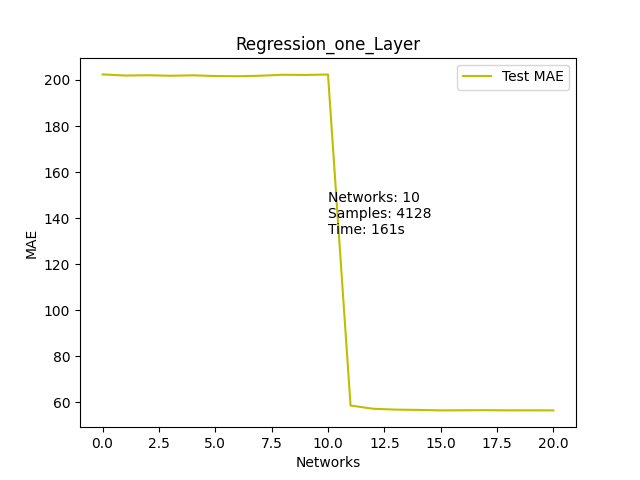
\includegraphics[height=5cm]{../../Plots/ba_plots/regression_large/onelayer_ts.png}
    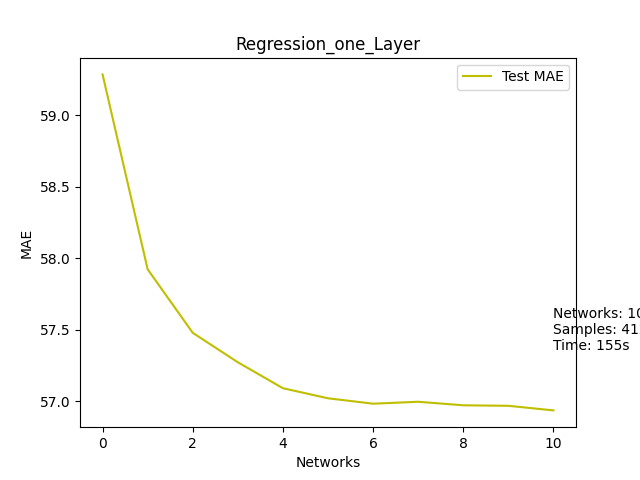
\includegraphics[height=5cm]{../../Plots/ba_plots/regression_large/woonelayer_ts.png}
    \caption{\label{fig:largeregr2} Vergleich im OneLayer Netzwerk}
\end{figure}

In Figure 5.2 ist das Ergebnis des Direct Cascade. Auf der linken Seite ist die Versioin mit TF. Dabei fällt auf, dass es bei vielen 
Targetdaten besser ist auf dem Targetdatensatz direkt zu lernen, denn 
das Wissen, welches vom Sourcedatensatz übertragen wird, ist nicht so passend, wie das von den Targetdaten. Dies passiert aber nur, wenn es 
genügend Targetdaten gibt. Bei diesem Vergleich kommen auch beim Deep Cascade ähnliche Werte heraus. 
Ein komplettes Netzwerk, wie es für Figure 5.3 genutzt wurde, hat etwa dieselbe Performanz, wie die beiden Kaskadenversionen. 

\begin{figure}[htpb]
    \centering
    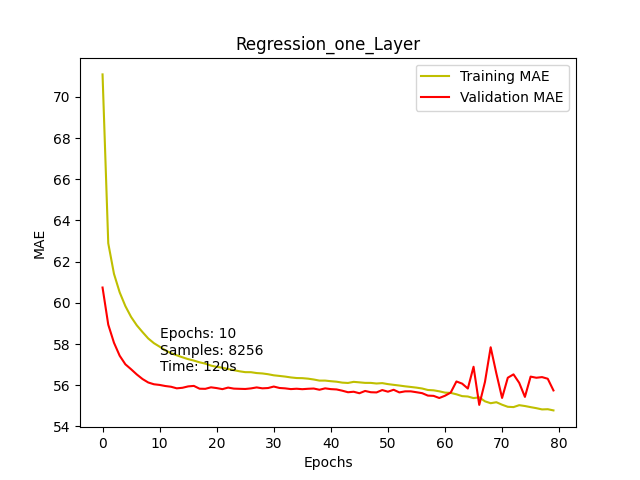
\includegraphics[height=5cm]{../../Plots/ba_plots/regression_large/onelayer_complete.png}
    \caption{\label{fig:largeregr2comp} Komplettes OneLayer}
\end{figure}

Dies liegt daran, dass die lineare Aktivierungsfunktion und der Mean Squared Error Loss für die Kaskadierung nicht störend sind. 
Also funktioniert Regression deutlich besser mit Kaskadennetzwerken als die Klassifikation, da sie an das Ergebnis des kompletten Netzes 
herankommt, was bei Klassifikation nie passiert ist. 
